\documentclass[a4paper,11pt]{article}
\usepackage[onehalfspacing]{setspace} %Zeilenabstand
\addtolength{\hoffset}{-2.25cm}
\addtolength{\textwidth}{4.5cm}
\addtolength{\voffset}{-3.25cm}
\addtolength{\textheight}{5cm}
\setlength{\parskip}{0pt}
\setlength{\parindent}{0in}

%----------------------------------------------------------------------------------------
%	PACKAGES AND OTHER DOCUMENT CONFIGURATIONS
%----------------------------------------------------------------------------------------

\usepackage{blindtext} % Package to generate dummy text
\usepackage{charter} % Use the Charter font
\usepackage[utf8]{inputenc} % Use UTF-8 encoding
\usepackage{microtype} % Slightly tweak font spacing for aesthetics
\usepackage[english, ngerman]{babel} % Language hyphenation and typographical rules
\usepackage{amsthm, amsmath, amssymb} % Mathematical typesetting
\usepackage{float} % Improved interface for floating objects
\usepackage[final, colorlinks = true, 
            linkcolor = black, 
            citecolor = black]{hyperref} % For hyperlinks in the PDF
\usepackage{graphicx, multicol} % Enhanced support for graphics
\usepackage{xcolor} % Driver-independent color extensions
\usepackage{marvosym, wasysym} % More symbols
\usepackage{rotating} % Rotation tools
\usepackage{censor} % Facilities for controlling restricted text
\usepackage{listings, style/lstlisting} % Environment for non-formatted code, !uses style file!
\usepackage{pseudocode} % Environment for specifying algorithms in a natural way
\usepackage{style/avm} % Environment for f-structures, !uses style file!
\usepackage{booktabs} % Enhances quality of tables
\usepackage{tikz-qtree} % Easy tree drawing tool
\tikzset{every tree node/.style={align=center,anchor=north},
         level distance=2cm} % Configuration for q-trees
\usepackage{style/btree} % Configuration for b-trees and b+-trees, !uses style file!
\usepackage{csquotes} % Context sensitive quotation facilities
\usepackage[yyyymmdd]{datetime} % Uses YEAR-MONTH-DAY format for dates
\renewcommand{\dateseparator}{-} % Sets dateseparator to '-'
\usepackage{fancyhdr} % Headers and footers
\pagestyle{fancy} % All pages have headers and footers
\fancyhead{}\renewcommand{\headrulewidth}{0pt} % Blank out the default header
\fancyfoot[L]{} % Custom footer text
\fancyfoot[C]{} % Custom footer text
\fancyfoot[R]{\thepage} % Custom footer text
\newcommand{\note}[1]{\marginpar{\scriptsize \textcolor{red}{#1}}} % Enables comments in red on margin

%----------------------------------------------------------------------------------------

\usepackage[english]{babel}
\usepackage{shellesc}
\usepackage{csquotes}
\usepackage[T1]{fontenc}
\usepackage{lmodern}
\usepackage{listings}
\usepackage{hyperref}
\usepackage[style=apa, backend=biber]{biblatex}
\addbibresource[]{ref.bib}
\renewcommand{\qed}{\hfill\blacksquare}
\newcommand{\qedwhite}{\hfill \ensuremath{\Box}}
\definecolor{answercolor}{HTML}{0071BC}
\newcommand*{\answer}{\textcolor{answercolor}}
\newenvironment{answerenv}{\color{answercolor}}{}
\newcommand{\E}{\mathbb{E}}
\newcommand{\pos}{\color{green} \uparrow \color{black}}
\newcommand{\negative}{\color{red} \downarrow \color{black}}
\usepackage{booktabs}
\usepackage{longtable}
\setcounter{section}{-1}
\usepackage{amsmath}
\usepackage{tikz}
\usetikzlibrary{arrows,calc}
\usepackage{relsize}
\usepackage{tcolorbox}
\newtcolorbox{qbox}[1]{colback=red!5!white, colframe=red!50!black, fonttitle=\bfseries,title=#1}

\begin{document}
\selectlanguage{english}
%-------------------------------
%	TITLE SECTION
%-------------------------------

\fancyhead[C]{}
\hrule  % Upper rule
\begin{minipage}{0.295\textwidth} 
\raggedright
\footnotesize
Lucas Paul Unterweger \hfill\\   
\hfill\\
Sophia Oberbrinkmann
\end{minipage}
\begin{minipage}{0.4\textwidth} 
\centering 
\large 
Assignment 2\\ 
\normalsize 
Adv. Macro II\\ 
\today \\
\end{minipage}
\begin{minipage}{0.295\textwidth} 
\raggedleft

\includegraphics[scale=0.15]{style/wu_transparent.png}\\
\end{minipage}
\hrule 
\bigskip

%-------------------------------
%	CONTENTS
%-------------------------------
\section{Preliminary}
We hereby declare that the answers to the given assignment are entirely our own, resulting from our own work effort only. Our team members contributed to the answers of the assignment in the following proportions: 
\begin{itemize}
	\renewcommand{\labelitemi}{$\Rightarrow$}
	\item Unterweger Lucas: 50\% 
	\item Oberbrinkmann Sophia: 50\%
\end{itemize}
\tableofcontents
\pagebreak
\listoffigures
%\listoftables
\pagebreak

\section{Transmission of monetary policy shocks (6 points)}
\begin{qbox}{\subsection{AS-AD Diagramm}}
Draw a diagram of an AS-AD model for the case of an AS curve with a mild upward slope. Do not forget to label all axes and curves. Now, consider the case of an expansionary monetary policy shock. Which curve shifts where (IS-LM diagram is not needed), and what are the effects on output and the price level? What happens in the short-run and what in the long-run? Why?
\end{qbox}
\textbf{Short run:}\\
 
An expansionary monetary policy shock can typically occur through a decrease in interest rates or an increase in the money supply through the central bank. This stimulates Investment and consumption which leads to an increase in aggregate demand. The AD curve shifts to the right which means an increase in the quantity of output demanded at each price level. In the short run, Output increases. The effect of the price level depends on the slope of the AS curve. In the short run, with a mild upward-sloping AS curve, the increase in aggregate demand will have a more significant impact on output than on the price level. Therefore, the primary effect is an increase in output, while the price level might experience a relatively moderate increase. \\

\textbf{Long run:} \\

Moving on to the long run, price expectations $P^e$ adjust abd as these prices adjust to the increased demand, the AS curve shifts upwards and the economy returns to its original output level. In the long run, the expansionary monetary policy shock primarily leads to an increase in the price level, with minimal impact in output. In the long run, the AS curve is assumed to become more vertical. This means that the economy's output is at a potential level and the price level is the main determinant of output in the long run. \\

\begin{figure}[H]
\centering
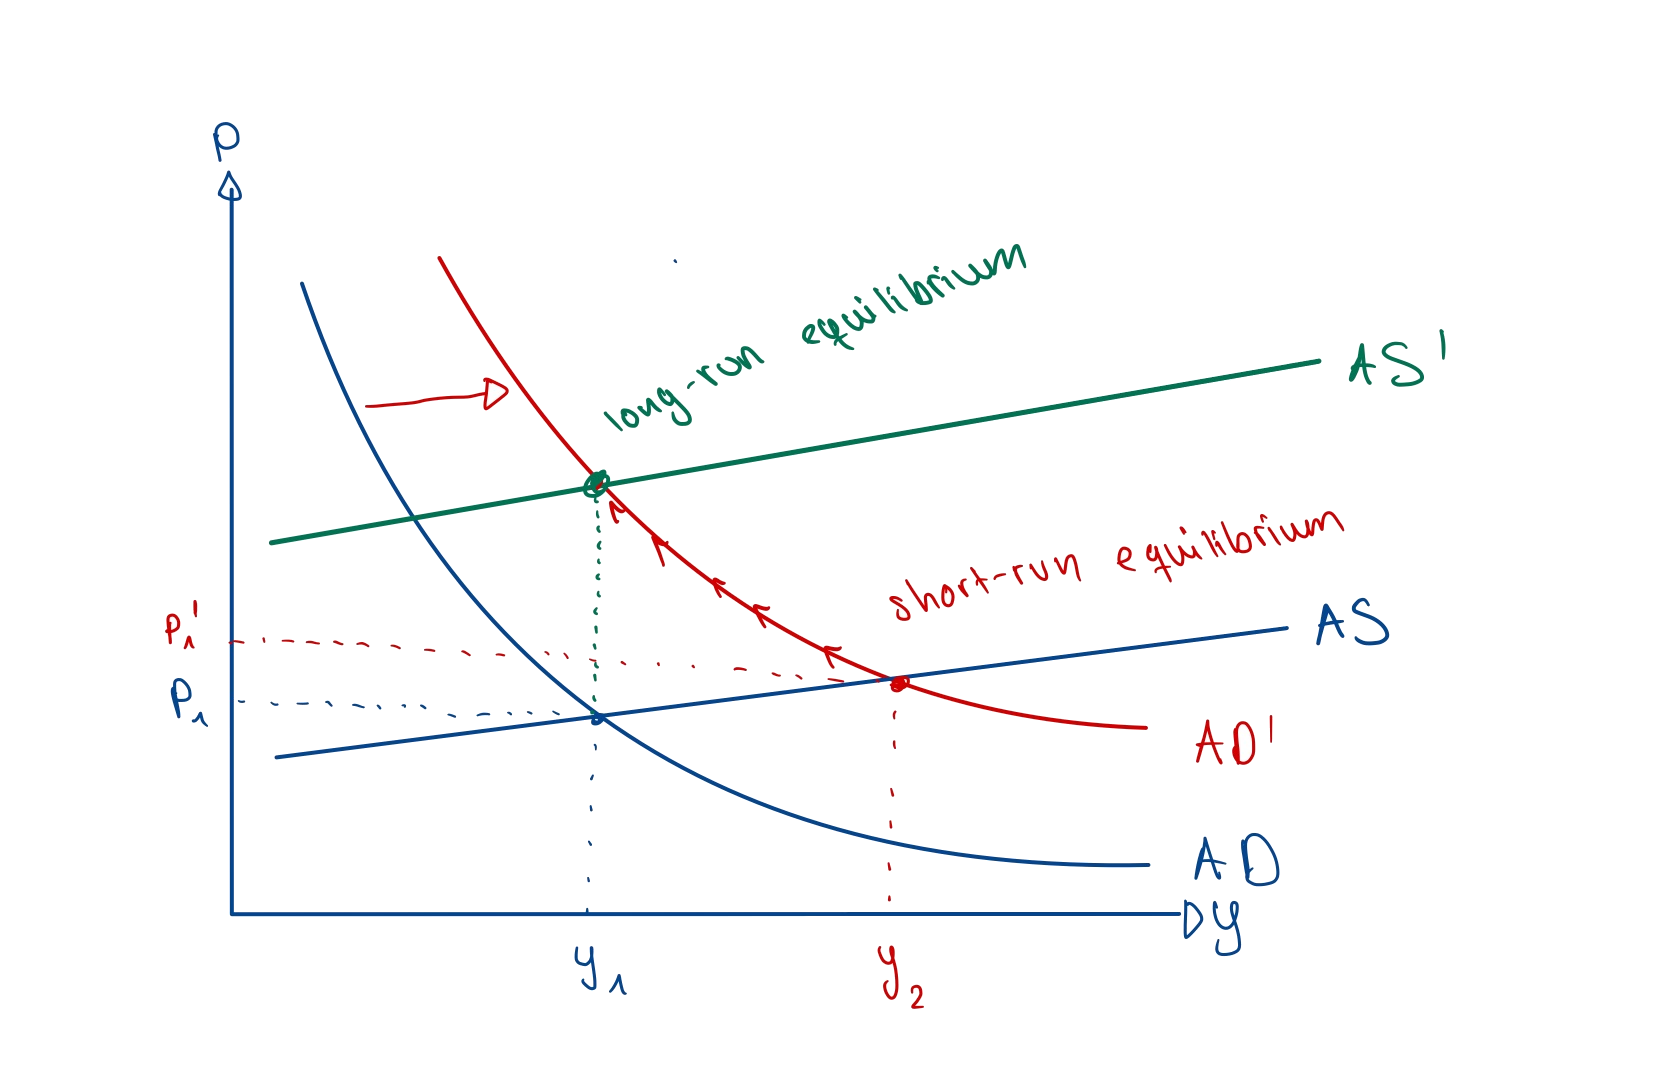
\includegraphics[scale=0.2]{figures/ASAD_mildslope.png}
\caption{Expansionary Monetary Policy Shock (Mild upward sloping AS) Note: $Y_1$ is meant to describe $Y_n$}
\end{figure}

\pagebreak

\begin{qbox}{\subsection{AS-AD cont'd}}
Redo the same as in exercise 1a) but with a with an AS curve that has a much steeper slope. Explain what are the di¤erences and why do they arise between the mild-slope case and the steep-slope case and how we can interpret them economically?
\end{qbox}

\textbf{Short run:}\\

Again an expansionary policy shock will lead to an increase in aggregate demand and the AD curve shifts to the right. With a steeper AS curve, the impact of the expansionary monetary policy shock on output and prices will differ from the mild slope case. In the short run, the expansionary policy shock will again lead to an increase in output, with rising aggregate demand. Compared to before the increase in output will be relatively smaller. In contrast the impact on the price level will be more significant than before. \\

\textbf{Long run:}\\

In the long run the steeper AS curve implies that the economy reaches it's potential output level much quicker. The impact on the price level will be more significant than before. \\

The differences arise from the degree of spare capacity in the economy. A mild-slope AS curve suggests that the economy has ample room to increase output within significant price increases. On the other hand, a steep slope AS curve indicates limited capacity, where increased demand leads to substantial price increase rather than output growth. These differences are important economically. In the steep sloped case expansionary monetary policy may be less effective in boosting output in the short run, but has a rather significant effect on the price level in both short and long run. \\

\begin{figure}[H]
\centering
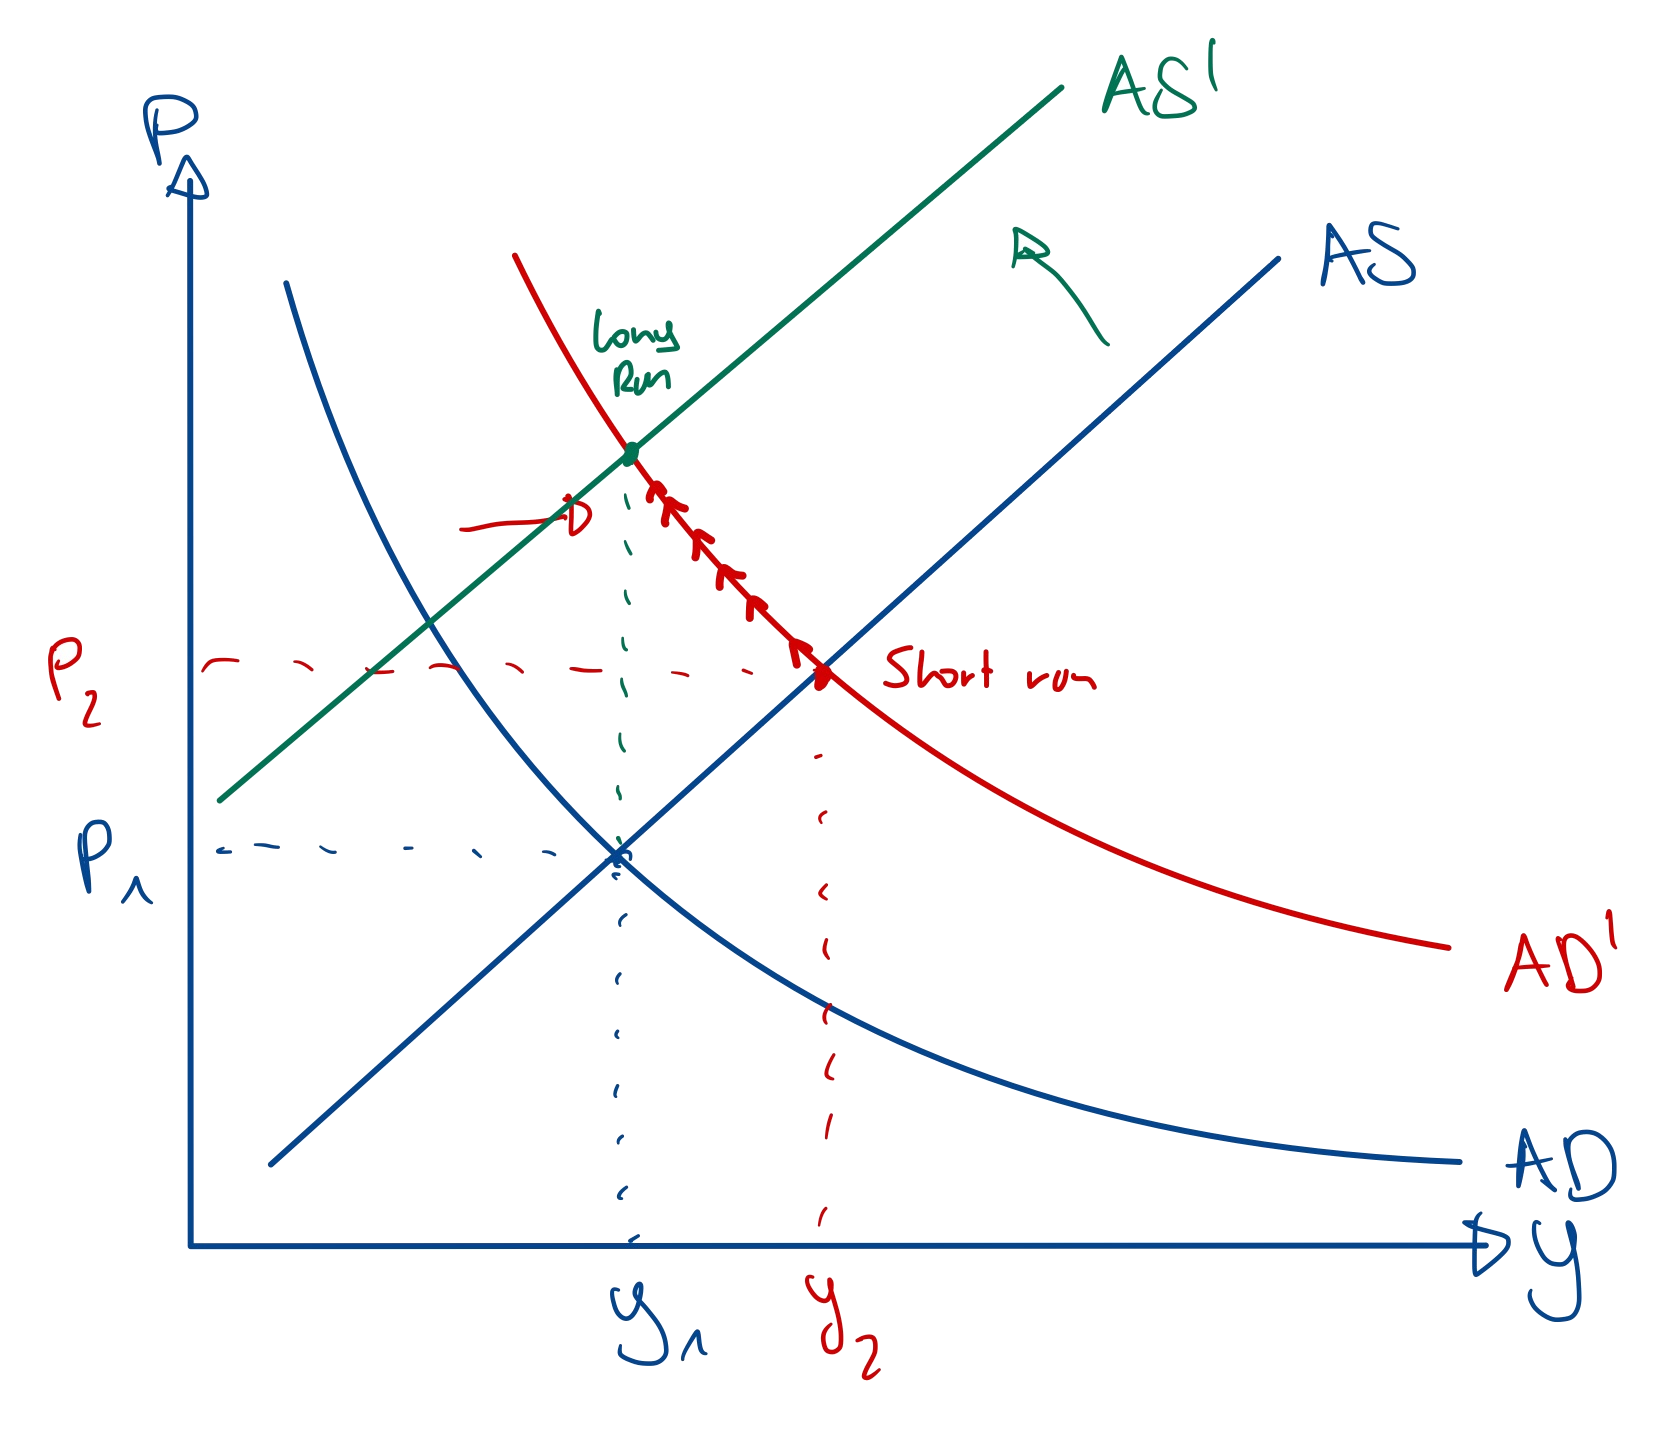
\includegraphics[scale=0.18]{figures/ASAD_steepslope.png}
\caption{Expansionary Monetary Policy Shock (Strong upward sloping AS) Note: $Y_1$ is meant to describe $Y_n$}
\end{figure}

\pagebreak

\begin{qbox}{\subsection{Implications of changes in the NK Model}}
Recall that the NKPC from the baseline New Keynesian model from class
is given by:
\begin{equation}
    \hat{\pi}_t = k(\hat{y}_t-\hat{y}_t^{flex})+\beta E_t \hat{\pi}_{t+1}
\end{equation}

where $k=\lambda (\sigma + \varphi)$, and where $\lambda = \frac{\theta-1}{\phi}$ under the assumption of Rotemberg price adjustment costs. What happens to the slope of the NKPC as prices become more fexible (lower price adjustment cost parameter $\phi$) or as market power of monopolistic competitors decreases (higher elasticity of substitution between varieties, $\theta$). How do your answers here relate to answers from question a.) and b.)? Under which parameter constellations (of $\phi$ and $\theta$) does monetary policy have large short-run effects?
\end{qbox}
\textbf{1) Prices become more flexible: the price adjustment cost parameter $\varphi$ falls.}\\ 

If prices become more flexible, it means that they can adjust more easily and quickly in response to changes in supply and demand conditions. 
The Parameter $k$ rises, which implies that prices adjust quicker in response to changes in the output gap. If prices become more flexible and the price adjustment parameter shirks, the slope of the NKPC would become steeper. \\

$$\negative \varphi \implies \pos\lambda = \frac{\theta-1}{\negative \varphi} \implies \pos k = \pos \lambda (\sigma + \phi) \implies \hat{\pi}_t = \pos k(\hat{y}_t-\hat{y}_t^{flex})+\beta E_t \hat{\pi}_{t+1}$$

\textbf{2) The market power of monopolistic competitors decreases, which means that there is higher elasticity of substitution between parameters. $\theta$ rises.  
The NKPC also becomes steeper as $k$ rises.} \\

If the NKPC becomes steeper, it implies that the relationship between inflation and the output gap becomes more sensitive. In relation to the AS-AD curve, the slope of the NKPC affects the short-run trade off between inflation and output. When the NKPC is steeper, it means that changes in the output gap will have stronger influence on inflation, which implies a steeper AS curve. Reducing phi and increasing theta is equivalent to the changes from a flatter AS curve to a steeper AS curve, as described in a) and b). 
A high phi and a low theta lead to stronger short-run effects, as the AS curve will be flatter. \\

$$\pos \theta \implies \pos\lambda = \frac{\pos \theta-1}{\varphi} \implies \pos k = \pos \lambda (\sigma + \phi) \implies \hat{\pi}_t = \pos k(\hat{y}_t-\hat{y}_t^{flex})+\beta E_t \hat{\pi}_{t+1}$$


\pagebreak

\section{A New Keynesian model with energy (11 points)}
Consider extending the New Keynesian model from class to include energy inputs needed for the production of goods. Luckily, nothing changes on the household side, so that the household problem and first order optimality conditions are fully described by slides 29-40 of lecture slides 2.
\begin{qbox}{\subsection{Firm side of the NKM}}
Now turn to the firm side. That is, firms are now assumed to produce using both labor and energy as production inputs, according to a Cobb-Douglas production function:
\begin{equation}
    Y_t(i) = A_tN_t(i)^{1-\alpha}EN_t(i)^\alpha
\end{equation}

The firm's dynamic problem continues to read:
\begin{equation}
    \max E_0\sum_{t=0}^\infty \Lambda_{0,t} \left[ P_t(i) Y_t(i) -MC_tY_t(i) - \frac{\varphi}{2}\left( \frac{P_t(i)}{P_{t-1}(i)}-1\right)^2P_tY_t\right],
\end{equation}

however, the definition of marginal cost, $MC_t$, has changed. For your convenience, you do not need to derive the dynamic FOC w.r.t. the choice of the optimal price, as this is identical as in the baseline NK model. Instead, you only need to solve the changed cost minimization problem below, which now requires deriving the first order conditions w.r.t. $N_t(i)$, $EN_t(i)$, and $MC_t(i)$:
\begin{equation}
    \min W_tN_t(i) + P_t^E EN_t(i) - MC_t(i)\left[ A_tN_t(i)^{1-\alpha}EN_t(i)^\alpha-Y_t(i)\right]
\end{equation}

where $P^E_t$ denotes the (nominal) price of energy, which we will take as exogenously given (i.e. we do not model a supply side for energy, and instead assume that energy is imported from abroad at price $P^E_t$).\\

Label the first order conditions of the above expenditure minimization problem w.r.t. $N_t(i)$, $EN_t(i)$, and $MC_t(i)$ equations eq1), eq2) and eq3).
\begin{itemize}
    \item Show that one can derive the optimal labor-to-energy ratio from combining equations eq1) and eq2), and that this ratio only depends on (aggregate) prices, so that the ratio is not firm-i specific.
    \item Show that one can derive an expression for marginal costs that also is the same for all firms i, by combining all three optimality conditions (that is, by expressing $N_t(i)$ from eq1 and $EN_t(i)$ from eq2 and plugging them in into the production function, eq3) to obtain the relevant expression for $MC_t(i)$ From now on, assume that all firms are identical, so that we can drop the i index.
\end{itemize}
\end{qbox}


%-------------------------------------------- Answer Question 2.1
We start by deriving the first order conditions. The FOC w.r.t $N_t(i)$ is given by
\begin{align*}
&\frac{\partial L}{\partial N_t(i)}  = W_t - MC_t(i)A_t (1-\alpha) N_t(i)^{-\alpha}EN_t(i)^\alpha \overset{!}{=} 0 \\
&\iff W_t = MC_t(i)A_t (1-\alpha) N_t(i)^{-\alpha}EN_t(i)^\alpha \\
&\iff MC_t(i) = \frac{W_t}{A_t (1-\alpha)N_t(i)^{-\alpha}EN_t(i)^\alpha}
\end{align*}

The first order condition w.r.t to $EN_t(i)$ is given by
\begin{align*}
&\frac{\partial L}{\partial EN_t(i)}  = P^E_t - MC_t(i)A_t N_t(i)^{1-\alpha}\alpha EN_t(i)^{\alpha-1} \overset{!}{=} 0 \\
&\iff P^E_t = MC_t(i)A_t N_t(i)^{1-\alpha}\alpha EN_t(i)^{\alpha-1} \\
&\iff MC_t(i) = \frac{P^E_t }{A_t N_t(i)^{1-\alpha}\alpha EN_t(i)^{\alpha-1}}
\end{align*}

The first order condition w.r.t to the marginal costs just results in the production function as can be seen belwo:
\begin{align*}
&\frac{\partial L}{\partial MC_t(i)}  = A_tN_t(i)^{1-\alpha}EN_t(i)^\alpha-Y_t(i) \overset{!}{=} 0 \\
&\iff Y_t(i) = A_tN_t(i)^{1-\alpha}EN_t(i)^\alpha
\end{align*}

The three FOC can thus be summarized as
\[
MC_t(i) = \frac{W_t}{A_t (1-\alpha)N_t(i)^{-\alpha}EN_t(i)^\alpha} \tag{eq1} \label{eq:eq1}
\]
\[
MC_t(i) = \frac{P^E_t }{A_t N_t(i)^{1-\alpha}\alpha EN_t(i)^{\alpha-1}} \tag{eq2} \label{eq:eq2}
\]
\[
Y_t(i) = A_tN_t(i)^{1-\alpha}EN_t(i)^\alpha \tag{eq3} \label{eq:eq3}
\]

\textbf{Labor-To-Energy Ratio}\\
By combining \eqref{eq:eq1} and \eqref{eq:eq2} we gain the optimal labor-to-energy ration using some simple algebraic rearrangement:\\
Rewrite \eqref{eq:eq1} as
$$MC_t(i)(1-\alpha) = \frac{W_t N_t(i)}{A_t N_t(i)^{1-\alpha}EN_t(i)^\alpha}$$
and \eqref{eq:eq2} as
$$A_t N_t(i)^{1-\alpha}EN_t(i)^{\alpha}= \frac{P^E_t EN_t(i)}{ \alpha MC_t(i)} $$
Now substituting \eqref{eq:eq2} into \eqref{eq:eq1} yields
\begin{align*}
    &MC_t(i)(1-\alpha) = \frac{W_t N_t(i) \alpha MC_t(i) }{P^E_t EN_t(i)}\\
    &\iff \frac{N_t(i)}{EN_t(i)} = \frac{1-\alpha}{\alpha} \frac{P^E_t}{W_t}
\end{align*}
It can clearly be seen that this ration is independent from the company specific index $i$.\\

\textbf{Marginal Costs}\\
To do this we'll make our lifes a bit easier by first incorporating \eqref{eq:eq3} into \eqref{eq:eq1} and \eqref{eq:eq2}. Using some basic algebraic manipulations we can see that
$$MC_t(i)(1-\alpha) = \frac{W_t N_t(i)}{A_t N_t(i)^{1-\alpha}EN_t(i)^\alpha} \implies MC_t(i)(1-\alpha) = \frac{W_t N_t(i)}{Y_t(i)}  \implies   N_t(i) = \frac{MC_t(i)(1-\alpha)Y_t(i)}{W_t}$$
as well as
$$A_t N_t(i)^{1-\alpha}EN_t(i)^{\alpha}= \frac{P^E_t EN_t(i)}{ \alpha MC_t(i)} \implies Y_t(i)= \frac{P^E_t EN_t(i)}{ \alpha MC_t(i)} \implies \frac{Y_t(i) \alpha MC_t(i)}{P^E_t} = EN_t(i)$$
Combining these two and substituting them into \eqref{eq:eq3} yields
\begin{align*}
    &Y_t(i) = A_tN_t(i)^{1-\alpha}EN_t(i)^\alpha = A_t\left( \frac{MC_t(i)(1-\alpha)Y_t(i)}{W_t}\right)^{1-\alpha} \left( \frac{Y_t(i) \alpha MC_t(i)}{P^E_t}\right)^\alpha \\
    \iff & Y_t(i) = MC_t(i) A_t (1-\alpha)^{1-\alpha}\alpha^\alpha Y_t(i)W^{\alpha-1}(P^E_t)^{-\alpha} \\
    \iff & 1 = MC_t(i) A_t (1-\alpha)^{1-\alpha}\alpha^\alpha W^{\alpha-1}(P^E_t)^{-\alpha} \\
    \iff & MC_t(i) = \frac{1}{A_t} \left( \frac{1}{1-\alpha}\right)^{1-\alpha} \left( \frac{1}{\alpha}\right)^\alpha W_t^{1-\alpha}(P^E_t)^{\alpha}
\end{align*}
which also shows the fact that the Marginal Costs $MC_t(i)$ are not dependent on the firm specific index $i$.

%-------------------------------------------- END Answer Question 2.1
%-------------------------- Question 2.2
\pagebreak
\begin{qbox}{\subsection{Non-linear Version of the energy-extended NK Model}}
Coding up the non-linear version of the energy-extended NK model: I uploaded dynare file NKmodelnonlin.mod on the Canvas course website. It codes up the baseline New Keynesian model from class (without energy), based on the set of non-linear first order and equilibrium conditions summarized on slides 65-66 of lecture slides 2, together with a basic feedback-to-inflation Taylor rule in its non-linear form, given by $(1+i_t)/(1+\Bar{i})=(\pi_t)^{\phi_\pi}e^{v_t}$. Use this file (and adopt the parameter values therein) as a basis to coding up the NK model with energy above. To do so, you only need to:
    \begin{itemize}
        \item exchange the expressions for the production function and marginal costs to the ones you found in 2a.)
        \item re-derive and replace the resource constraint, by following the steps layed out on slide 50 of the lecture notes and using the appropriate  expression for (real) profi ts of the above energy-NK model,
        $$\frac{\Pi_t}{P_t} = Y_t - \frac{W_t}{P_t}N_t - \frac{P^E_t}{P_t}EN_t - \frac{\varphi}{2}\left(\pi_t-1\right)^2Y_t$$
        \item add the optimal labor-energy ratio derived in 2a.) to your system of equations
        \item add the exogenous law of motion for the energy price to your system. This exogenous process is given for the real energy price $p^E_t = \frac{P^E_t}{P_t}$ and reads:
        $$\log p^E_t = \rho_{PE} \log p^E_{t-1}+\epsilon_{pe,t}$$
        \item assign the following additional model parameters in the energy-extended NK model: $\alpha = 0.05, \rho_{PE} = 0.5$. Else leave all other parameters as in file NKmodelnonlin.mod.
    \end{itemize}
\end{qbox}

As in the previous assignment, our code can be found on \href{https://github.com/therealLucasPaul/AdvMacroeconomics2_Assignments}{GitHub} or in the Appendix. Using the previously derived equations will us the recommended procedure and substitute the production function and the marginal costs with the following equations. For convenience, we also rewrote the equations for marginal costs, wage and energy price in real terms. 
\begin{align*}
&Y_t(i) = A_tN_t(i)^{1-\alpha}EN_t(i)^\alpha \\
&MC_t(i) = \frac{1}{A_t} \left( \frac{1}{1-\alpha}\right)^{1-\alpha} \left( \frac{1}{\alpha}\right)^\alpha W_t^{1-\alpha}(P^E_t)^{\alpha}\\
&\iff \frac{MC_t(i)}{P_t} = \frac{1}{A_t} \left( \frac{1}{1-\alpha}\right)^{1-\alpha} \left( \frac{1}{\alpha}\right)^\alpha \left(\frac{W_t}{P_t}\right)^{1-\alpha}\left(\frac{P^E_t}{P_t}\right)^{\alpha}
\end{align*}
Also, we re-derived the resource constraint as
\begin{align*}
&C_t = \frac{W_t}{P_t}N_t + \frac{T_t}{P_t} \\
\iff &C_t = \frac{W_t}{P_t}N_t + Y_t - \frac{W_t}{P_t}N_t-\frac{P^E_t}{P_t}EN_t - \frac{\phi}{2}(\pi_t-1)^2Y_t\\ 
\iff &C_t = Y_t -\frac{P^E_t}{P_t}EN_t - \frac{\phi}{2}(\pi_t-1)^2Y_t
\end{align*}

The optimal labor-to-energy ratio can also be rewritten in real terms to gain
$$\frac{N_t(i)}{EN_t(i)} = \frac{1-\alpha}{\alpha} \frac{P^E_t}{W_t} = \frac{1-\alpha}{\alpha} \frac{P^E_t/P_t}{W_t/P_t}$$

Finally, by adding the exogenous law of motion for the energy price and by adjusting the parameter values we gain the desired result. Again, the final code can be found on Github and the Appendix.\\

\pagebreak

\begin{qbox}{\subsection{Impulse Response Functions}}
Derive impulse reponses to i) a monetary policy shock and ii) a technology shock. How do they qualitatively differ from the baseline model we have seen in class? Also, iii) present impulse responses to a energy price shock and discuss what and why happens to the macroeconomy.
\end{qbox}

Using the code from the subsection before we derived Impulse Response Functions (IRFs) for monetary policy, technology and energy price shocks.
\subsubsection{Monetary Policy Shock}
\begin{figure}[H]
\centering
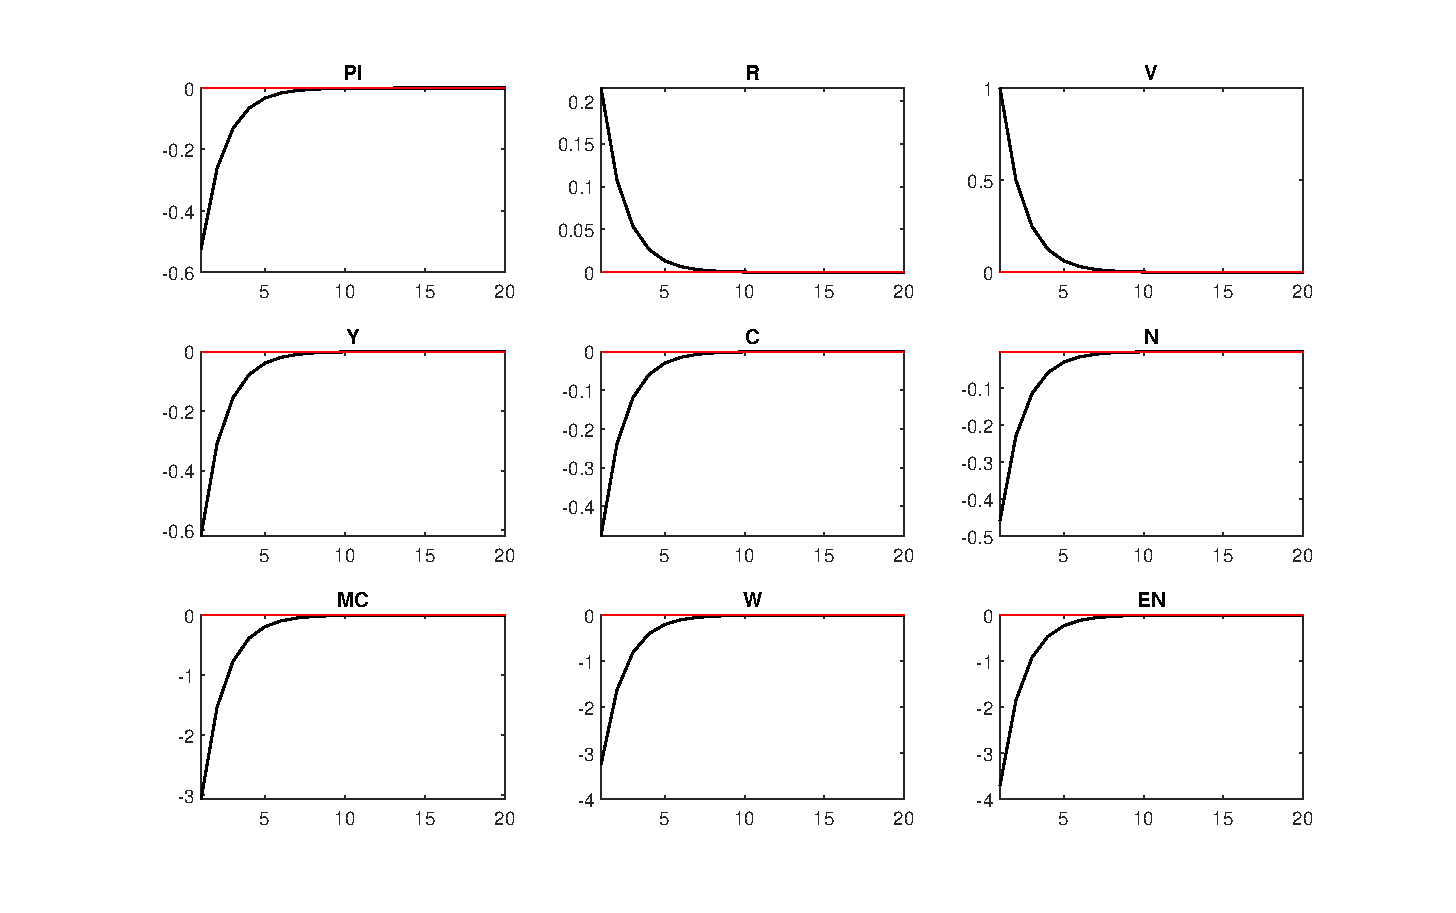
\includegraphics[scale=0.7]{figures/monpolshock.eps}
\caption{Monetary Policy Unit Shock}
\end{figure}
Similar to the case we had a look at in class, we will look at a 1\% monetary policy shock. Overall, the various effects are very similar in the scenario where we included energy prices. The monetary policy shock increases the nominal interest rate via $v$ and thus prices decrease, which can be seen in the IRF of the inflation variable, but not by as much as the nominal interest rate increases. This, in turn, causes the real interest rate $r$ to increase, which leads to a fall in consumption. Output and labour thus in turn follow a similar movement as in class. The most interesting fact here can be seen from the size of the effects. The 1\% interest rate shock causes the employment to fall, but not as much as in the baseline NK model as the drop in output can also be realized by decreasing the energy input which has a much smaller return to scale due to the $\alpha$ being $0.05$. That's why is more efficient to - in relative terms - decrease the less efficient energy input. However, qualitatively the effects are very similar to the ones from the baseline model. 

\subsubsection{Technology Shock}
\begin{figure}[H]
\centering
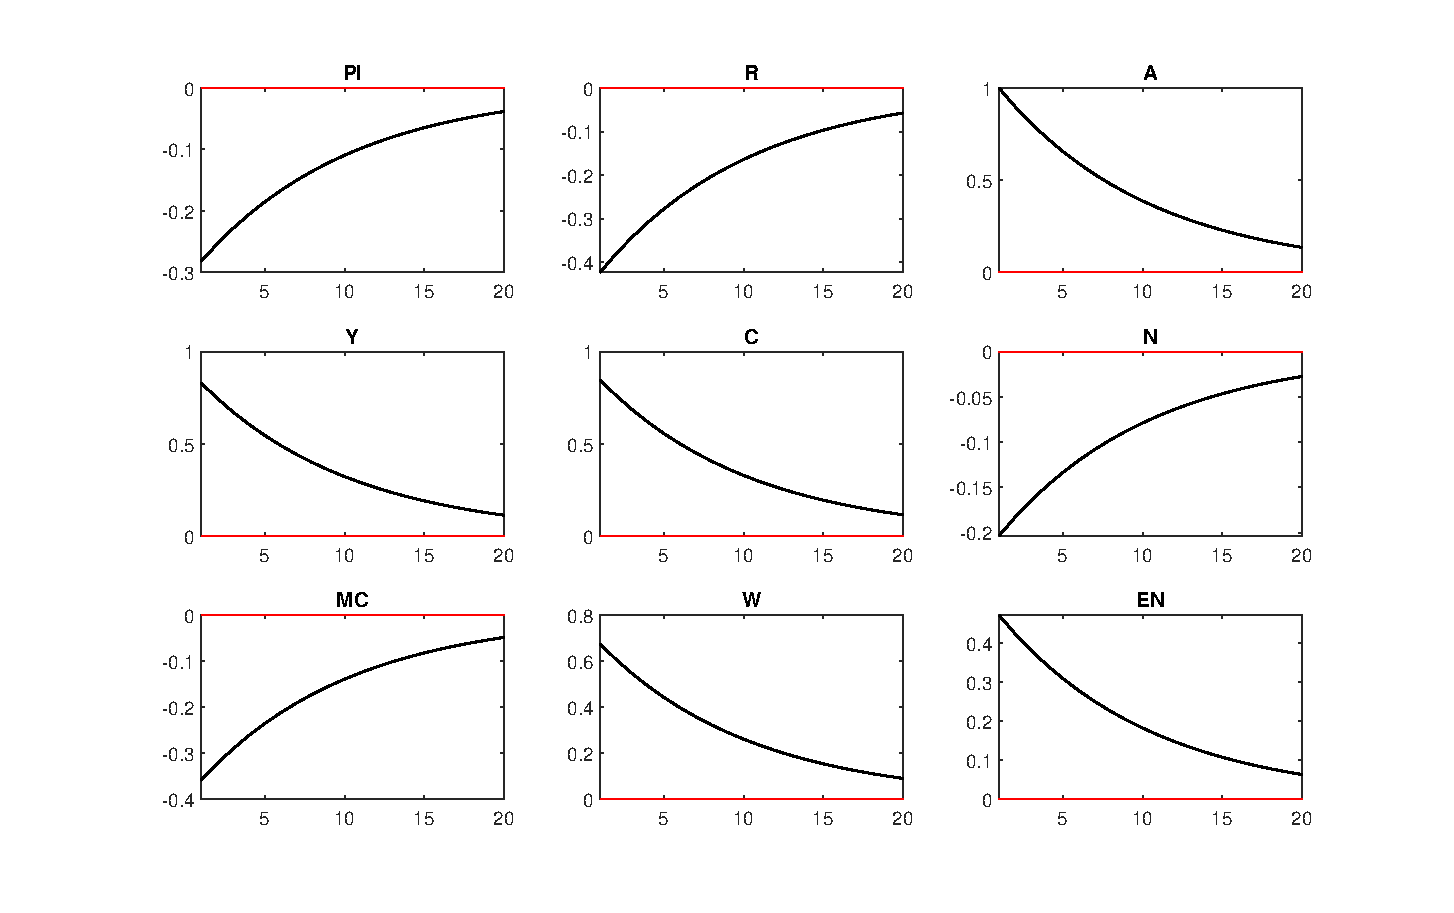
\includegraphics[scale=0.7]{figures/techshock.eps}
\caption{Technology Unit Shock}
\label{fig:techshock}
\end{figure}
Again, we will have a look at the 1\% unity shock to TFP, which can be seen in the upper right panel in figure \ref{fig:techshock}. The increase in TFP has a negative effect on the marginal costs, because firms can now produce their goods in a more efficient manner, which can also be seen from the marginal costs equation from above. This has a negative effect on inflation and the central bank adjusts according to the Taylor rule by decreasing the nominal interest rate such that the real interest rate also decreases. The households can now purchase more goods (consume more) and the firms increase the output. Qualitatively we they do not differ to the baseline case.   

\subsubsection{Energy Price Shock}
\begin{figure}[H]
\centering
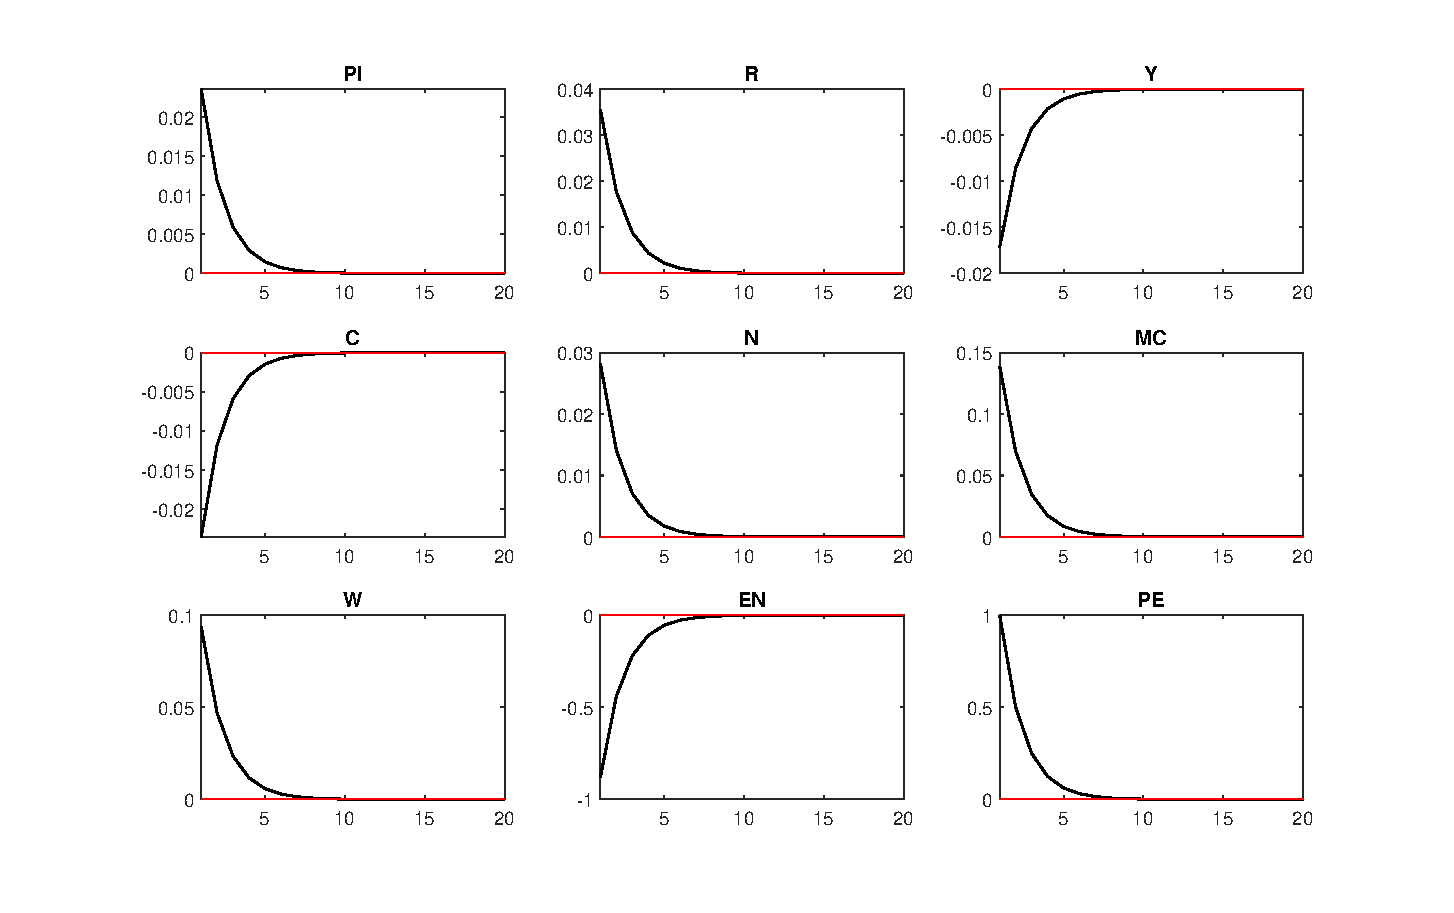
\includegraphics[scale=0.7]{figures/enpriceshock.eps}
\caption{Energy Price Unit Shock}
\label{fig:enpriceshock}
\end{figure}
Now, we will analyse a 1\% energy price shock to the economy. This effect can be seen from the lower right panel in figure \ref{fig:enpriceshock}. 

The first effect that can be seen is that the marginal costs increase due to the increase in real energy prices. This effect can also be seen from the marginal cost equation from above, which displays the positive relationship between marginal costs and the real energy price. Due to this increase, the inflation increase and the central bank - based on the Taylor rule - increases the nominal interest rate (stronger than the increase in inflation). Thus, the real interest rate also increases. The higher real interest rate leads to a fall in consumption, which in turn leads to a lower demand for output. Due to the fact that energy has become relatively more expensive than before, we can see that the labour input increases slightly and the energy input decreases. The resulting increase in real wages also has a positive effect on the aforementioned marginal costs. 

Overall, we can see that the energy price shock has an immediate effect on the macroeconomy. The higher input price leads to higher inflation and an immediate reduction in the overall output of economy, because the demand decreases and firms adjust. Nevertheless, the firms also try to adjust to the higher energy prices and substitute energy for labour input (the wages increase less than the energy price). This is a scenario which is quite visible in the current economic situation caused by the Russian invasion of Ukraine, where a massive gas price shock lead to similar effects.   

\section{Policy Application (5.5 points)}
\begin{qbox}{\subsection{Essay}}
Listen to the interview of Ricardo Reis (LSE) on VoxEU on "How did inflation get so high?" (\href{https://cepr.org/multimedia/how-did-inflation-get-so-high}{Link}). In a brief statement or mini-essay of about 300 words (e.g., suppose you work at a central bank and need to consult/brief your superior/governor), talk about a key insight or interesting aspect that you take.
\end{qbox}

The Interview with Ricardo Reis provides some insights about some possible reasons for the burst of high inflation in 2021/22. He highlights some hypotheses that could explain this phenomenon. One key aspect that stands out is the role of expectations and their influence on monetary policy effectiveness. \\

In the baseline New Keynesian model, we have learned that expectations play a crucial role in shaping inflation dynamics and the transmission of monetary policy. The model assumes that households and firms have rational expectations and form their beliefs about future inflation based on available information. The central bank’s ability to anchor inflation expectations is seen as a key determinant of its success in achieving its goals, most prominently maintaining price stability. \\

Reis suggests that one of the reasons for the high inflation experienced in 2021/22 was a neglect of expectations data. Central banks may have believed - and many political and economic institutions hoped - that inflation expectations were firmly anchored and that any increases in inflation would be temporary. This implies a potential deviation from the assumption of the New Keynesian model, where anchored expectations are essential for monetary policy effectiveness. In other words, the central bank might have missed on acting according to the Taylor Rule, which would have suggested to implement an early and strong increase in the key interest rates.\\

Additionally, Reis points to the over-reliance on past credibility as a factor that may have contributed to the burst of high inflation. In general, central banks earn credibility through their commitment to price stability and the successful implementation of necessary monetary policy. However, Reis suggests that relying too heavily on past credibility can create an illusion of room for focusing on real activity recovery while underpredicting the resulting inflation. This highlights the importance of constantly reassessing the changing economic environment and not solely relying on past successes to keep a central banks ability to efficiently effect real key variables. \\

The last point he made was regarding a revision of strategy that made central banks tolerant of higher inflation due to the trend fall in the return of government bonds. This aspect induces considerations beyond the New Keynesian model, such as the impact of changing financial conditions and the role of the private capital market. \\

All in all, Reis emphasizes the significance of expectations, credibility, and the interaction between monetary policy and financial conditions in understanding the reasons for high inflation. While these insights roughly align with elements of the baseline New Keynesian model, they also go beyond it by incorporating factors that are not explicitly modelled in the standard framework. \\
 
\pagebreak

\section{Appendix}
\subsection{Dynare Code}
\lstinputlisting[language=Matlab]{NKmodel_nonlin_Abgabe.mod}
\end{document}
